% Rafael Sartori M. dos Santos, 186154
\documentclass[brazilian,a4paper,twocolumn]{article}

% Título
\title{MC920 -- Trabalho 1}
\author{Rafael Sartori M. Santos, 186154}
\date{11 de setembro de 2019}

% Configuração do documento
\setlength{\parskip}{3pt}
\usepackage[utf8]{inputenc} % tipo de documento UTF-8
\usepackage{mathtools} % permitir expressões matemáticas
\usepackage{babel} % configuração da lingua portuguesa
\usepackage{caption} % para legenda de tabelas e figuras
\usepackage[
    pdfauthor={Rafael Sartori M. Santos},
    pdftitle={Trabalho 1 -- MC920},
    pdfproducer={LaTeX (texlive) com hyperref}
]{hyperref} % para links externos (href)
\usepackage{cleveref} % para referenciar tabelas e figuras melhor
\usepackage{indentfirst} % indentação de todo primeiro parágrafo
\usepackage{graphicx} % para adicionar imagens
\usepackage{subcaption} % para imagens ficarem lado a lado
% Usamos geometry pois dá mais espaço que fullpage
%\usepackage{geometry} % alterar geometria do papel
%\geometry{a4paper,left=1.7cm,right=1.7cm,top=1cm,bottom=2.0cm} % menor margem
\usepackage{fullpage} % utilizamos uma versão com menos espaçamento nas bordas

% Início do documento
\begin{document}

\maketitle

\section{Introdução}

    O objetivo do trabalho é analisar, no processo de \textit{half-toning}, os diferentes métodos de difusão de erro: Floyd-Steinberg, Sevenson-Arce, Burkes, Sierra, Stucki e Jarvis-Judice-Ninke. Aplicarei uma transformação em 2 níveis para cada camada de cor de uma imagem representada com 3 camadas: vermelho, verde e azul (R, G, B). Obteremos ao final $8$ possibilidades de cor para cada ponto da imagem. Analisarei uma imagem de grande dimensão no formato PNG quanto a sua semelhança à original em uma tela de computador em 2 casos: curta e longa distância de visualização.

    Farei esse processamento utilizando Python com as bibliotecas \href{https://opencv.org/}{\emph{OpenCV}} e \href{https://numpy.org/}{\emph{NumPy}} em um \href{https://jupyter.org/}{\emph{Jupyter Notebook}}.


\section{Método}

    Capturei uma imagem de grande dimensão (3096x4128) colorida com meu celular sob condições de alta luminosidade, pois gostaria de avaliar o efeito produzido em imagens que são comuns ao dia a dia. Converti do formato original JPEG para PNG utilizando a ferramenta \href{https://www.gimp.org/}{\emph{GIMP}}. No tratamento, utilizo apenas a PNG para não possuir intererência da compressão com perdas do outro formato.

    Para realizar o processamento digital, as bibliotecas de Python que utilizei foram:
    \begin{itemize}
        \item \emph{OpenCV} para abrir e salvar imagens;
        \item \emph{NumPy} para aplicar transformações à imagem;
        \item Alguns módulos da padrão para calcular tempo de execução e iterar de formas diferentes na imagem.
    \end{itemize}
    Organizei todo código responsável pelo processamento e medição de tempo em um \emph{Jupyter Notebook}; o que era responsável por abrir e salvar imagens e aplicar as conversões necessárias para utilizar nas bibliotecas em um módulo de utilidade (comum a outros trabalhos da disciplina).

    Escolhi manter apenas 2 níveis de intensidade para cada camada de cor da imagem. Como há 3 camadas na imagem testada, obtive $ 2^3 $ possibilidades de cores para cada ponto. Apesar disso, o código não é limitado quanto ao número de camadas.

    \subsection{Meios-tons}

        Começo separando as camadas da imagem colorida de $N$ camadas de cores em $N$ matrizes de dimensões iguais (uma para cada cor). A aplicação de meios-tons na camada $f$ para produzir a camada $g$ é dada pela \cref{eq:meios-tons}.

        \begin{equation}
        \label{eq:meios-tons}
            g(x, y) =
            \begin{cases}
                255     & \text{se $f(x, y) \geq 128$} \\
                0       & \text{caso contrário}
            \end{cases}
        \end{equation}

        Podemos realizar essa operação de forma vetorial apenas quando nenhuma difusão de erro é aplicada.

    \subsection{Aplicação da difusão de erro}

        Represento cada método de difusão através de uma matriz, que chamarei simplesmente de filtro, cujo centro de aplicação deve ser mencionado para sabermos onde aplicá-lo de forma vetorial. A difusão de Floyd-Steinberg, por exemplo, é representada pelo par matriz e centro de aplicação:
        \begin{equation*}
            \Bigg(
            \begin{bmatrix}
                0 & 0 & 7/16 \\
                3/16 & 5/16 & 1/16
            \end{bmatrix}
            ,\; (0, 1)
            \Bigg)
        \end{equation*}

        Para fazermos a aplicação de forma ainda mais efiicente, que é necessário pelo tamanho da imagem, precisamos adicionar \textit{padding} na imagem de entrada. O tamanho da borda é o mínimo necessário (calculado a partir do tamanho do filtro) para que o filtro possa ser aplicado sem condicionais.

        Para percorrer a imagem, criei um \textit{iterator} para a imagem que realiza o zigue-zague na imagem como recomendado para a atividade: em linhas ímpares, percorremos a imagem crescentemente; nas pares, decrescentemente. Ele retorna em cada ponto a tupla composta pela coordenada horizontal, vertical e ainda o filtro, que é espelhado em relação à vertical nas linhas pares.

        O \textit{iterator} é implementado de forma a reduzir os condicionais necessários enquanto navega a imagem através de ponteiro para função que é chamada a cada iteração, atualizada a cada linha. Outro benefício de utilizar essa interface é facilitar a implementação de outros caminhos: basta substituir o \textit{iterador}.

    \subsection{Limitações}

        Como, para disseminar erros, é necessário alterar a imagem de entrada na aplicação, não é possível vetorizar toda a aplicação do filtro na imagem. Por conta isso, só consegui vetorizar a aplicação da difusão de erro em cada ponto da imagem e a correção de valores (para manter a imagem no intervalo $[0, 255]$ quando é armazenada em \textit{$8$ bits}). Isso resulta em um código que demora vários minutos para imagens grandes: para que utilizei, por exemplo, o tempo de execução foi entre $879,98$ e $918,84$ segundos (aproximadamente $15$ minutos) para cada filtro.

        Vale ressaltar que tentei executar em paralelo o processamento de cada camada utilizando a biblioteca padrão \texttt{multiprocessing}, mas houve problemas de compartilhamento de memória entre processos quando a imagem possui grandes dimensões. Alguma bibliotecas não-padrão de Python poderia solucionar isso.


\section{Resultados obtidos e análise}

    Há algumas considerações que valem para todas as imagens. Por exemplo, apesar da abordagem que utilizo para aplicação do filtro alterar a borda, perdendo valores que poderiam ser mantidas na imagem com outras soluções, não foi possível notar algum artefato específico às bordas nas respostas.


    \subsection{Binarização sem difusão de erro}

        A simples binarização, mostrada na \cref{fig:binarizada-sem_difusao}, dada apenas pela \cref{eq:meios-tons}, é ineficiente sozinha: há grandes distorções em todas as cores e perda de detalhes causada pela consideração de apenas um ponto para o cálculo do ponto na imagem resultante.

        \begin{figure}
            \centering
            \begin{subfigure}{0.24\textwidth}
                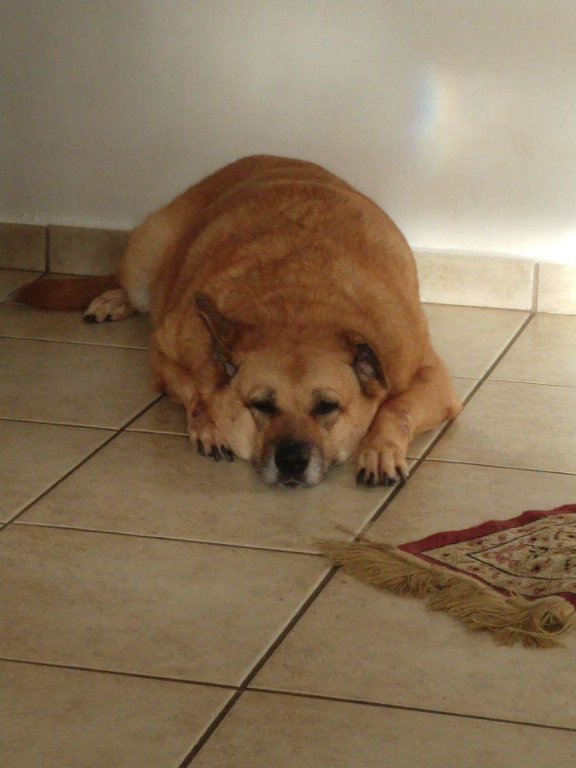
\includegraphics[width=\textwidth,keepaspectratio]{../imgs/mel.png}
                \caption{Imagem original}
            \end{subfigure}
            \begin{subfigure}{0.24\textwidth}
                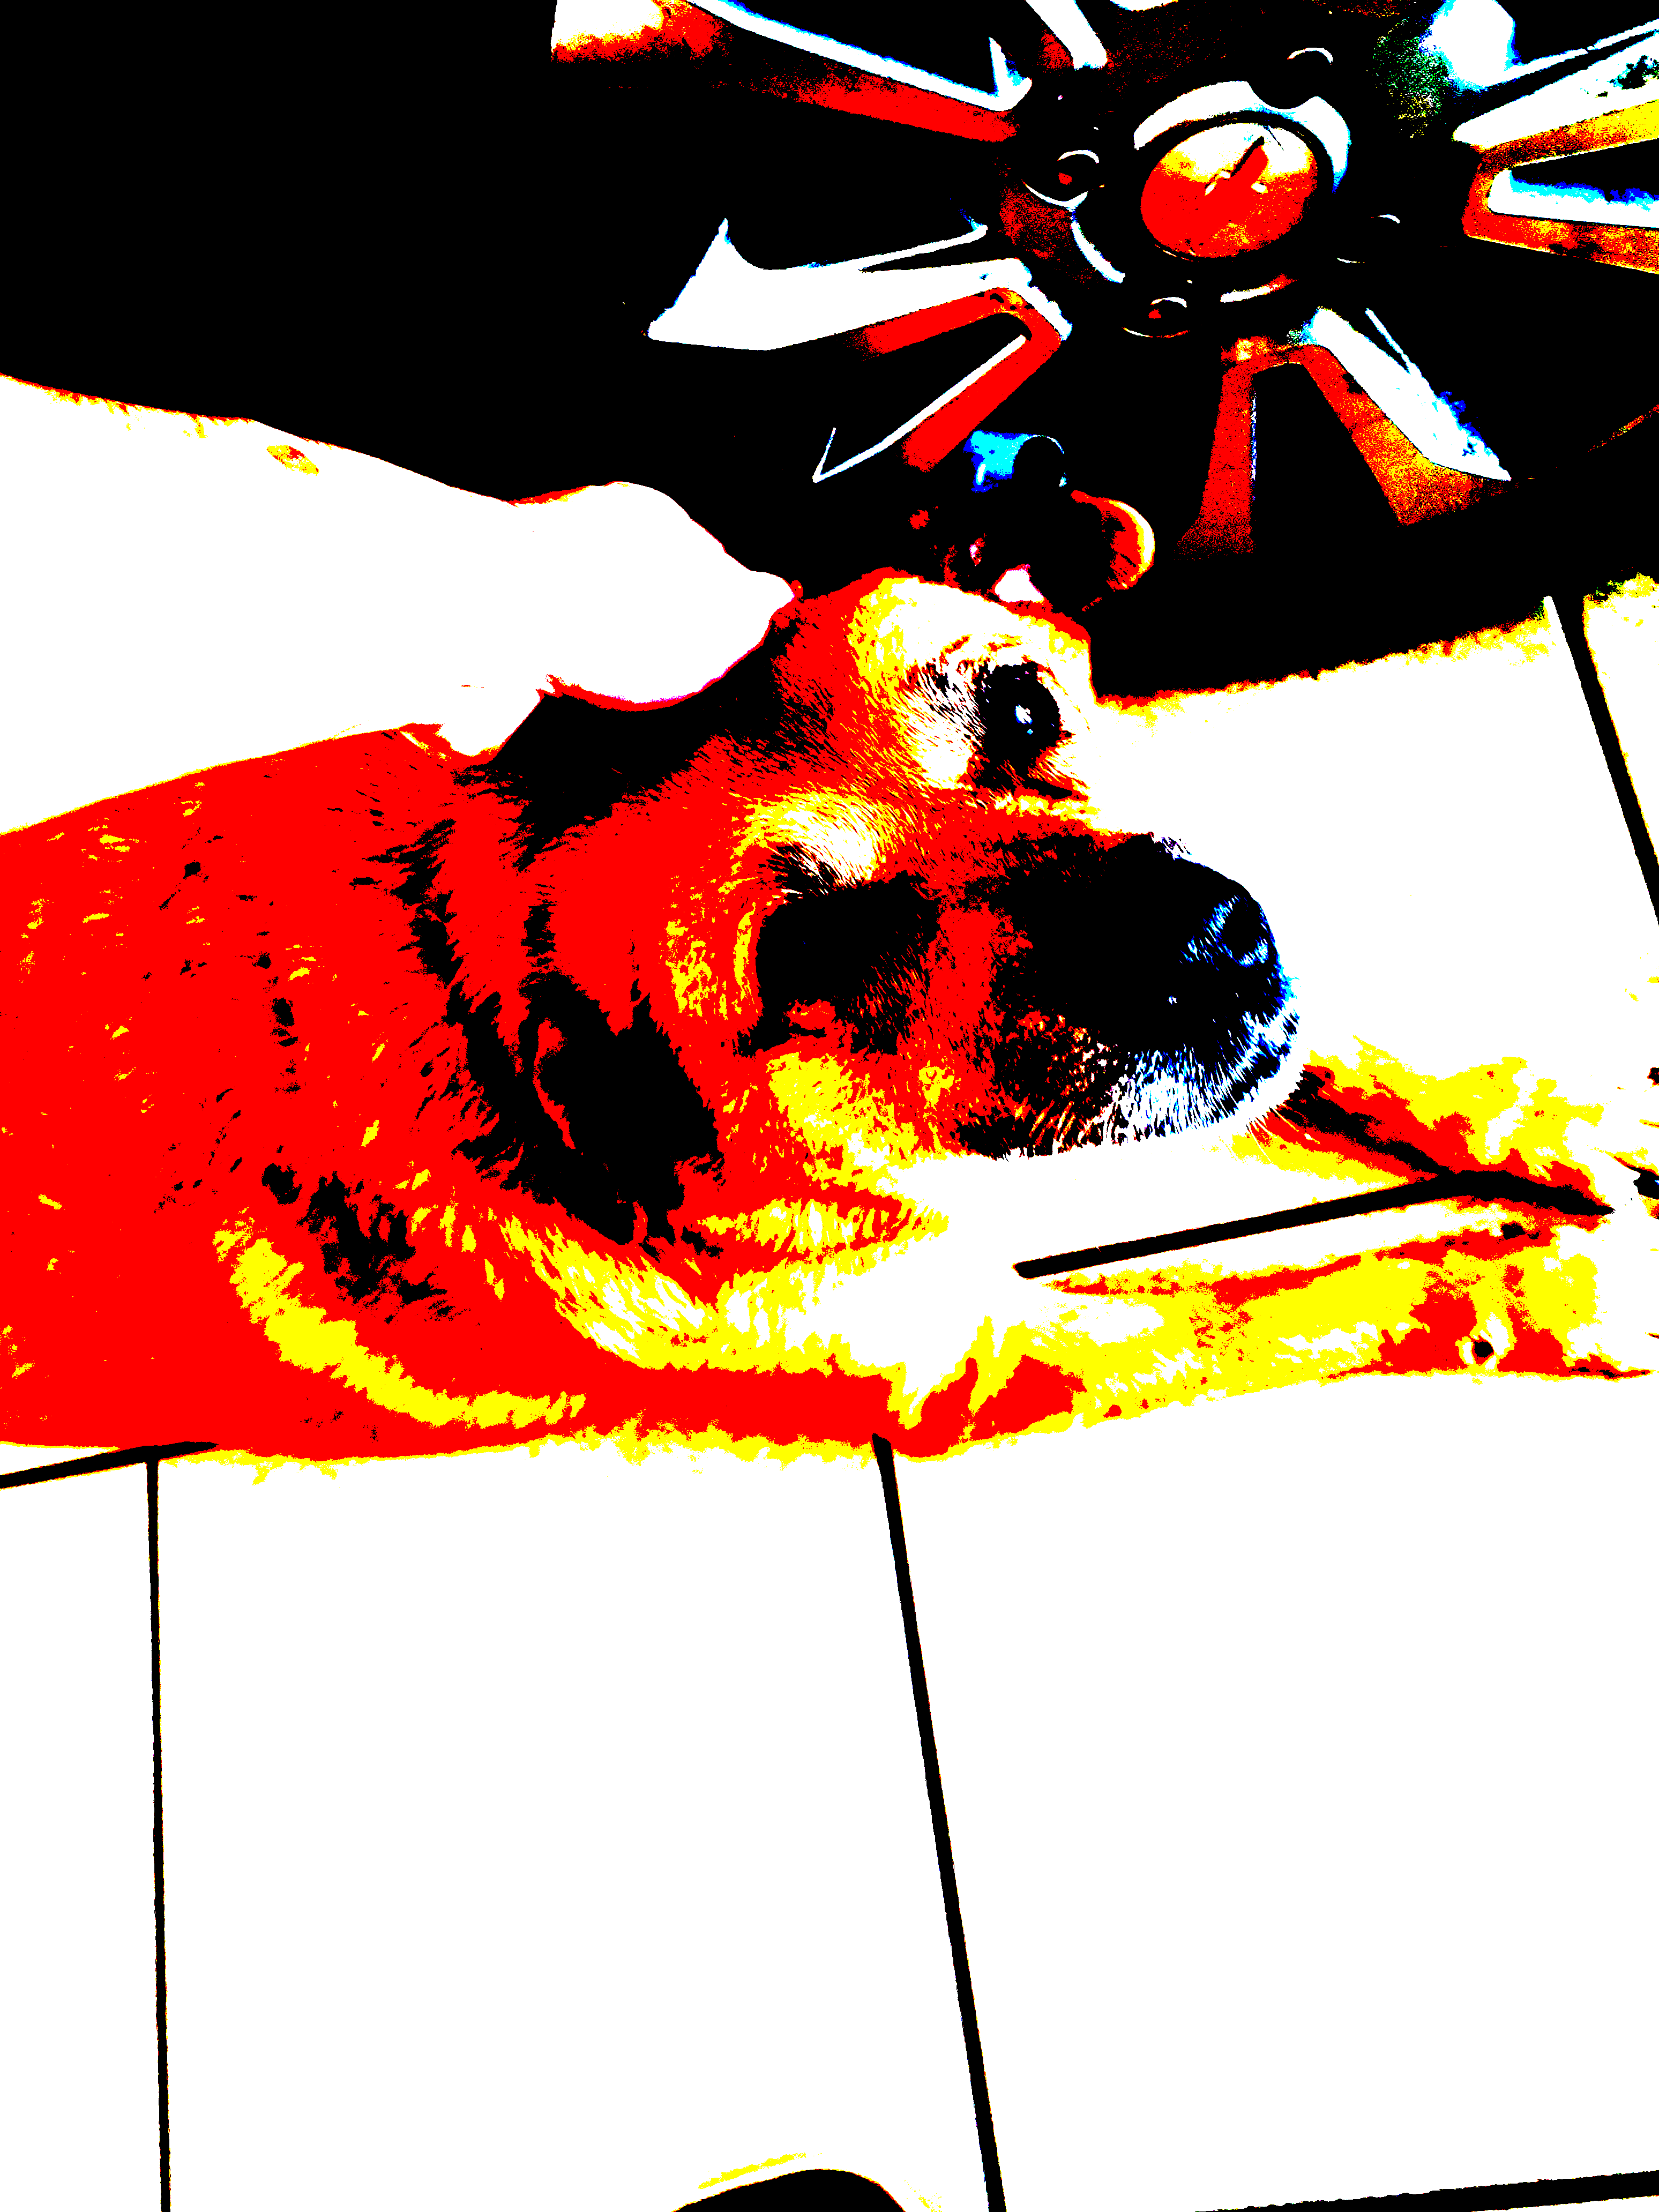
\includegraphics[width=\textwidth,keepaspectratio]{../imgs/mel-binarizada.png}
                \caption{Imagem binarizada sem difusão de erro}
            \end{subfigure}

            \caption{Comparativo para binarização sem difusão}
            \label{fig:binarizada-sem_difusao}
        \end{figure}

    \subsection{Difusão de erro de Floyd-Steinberg}

        A difusão de Floyd-Steinberg, mostrada na \cref{fig:binarizada-floyd_steinberg}, apesar de ser uma melhora considerável quando comparado com a binarização simples, apresenta um destaque grande às linhas de 45 graus.

        Essas linhas são a causa das distorções de cores acentuadas,

        \begin{figure}
            \centering
            \begin{subfigure}{0.24\textwidth}
                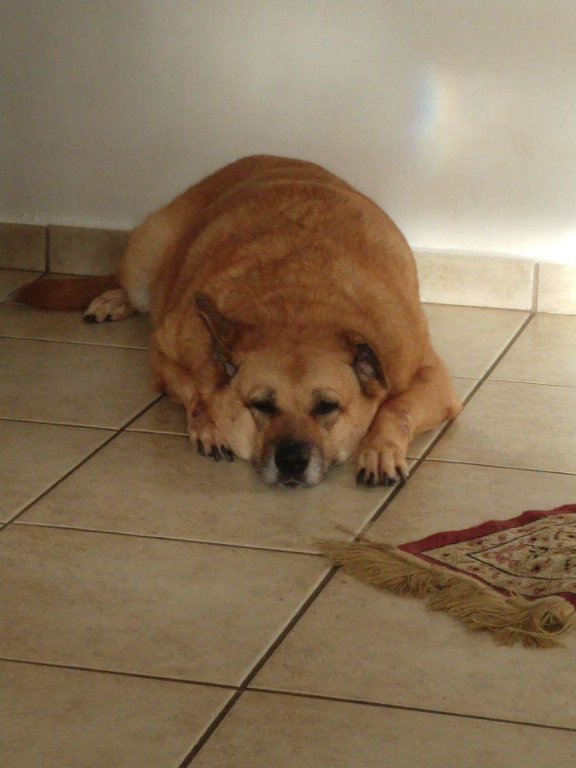
\includegraphics[width=\textwidth,keepaspectratio]{../imgs/mel.png}
                \caption{Imagem original}
            \end{subfigure}
            \begin{subfigure}{0.24\textwidth}
                \includegraphics[width=\textwidth,keepaspectratio]{../imgs/mel_binarizada-floyd_steinberg.png}
                \caption{Imagem com difusão de erro Floyd-Steinberg}
            \end{subfigure}

            \caption{Comparativo para binarização com difusão de erro de Floyd-Steinberg}
            \label{fig:binarizada-floyd_steinberg}
        \end{figure}

    \subsection{Difusão de erro de Burkes}

        A difusão de Burkes possui os mesmos problemas que as de Floyd-Steinberg, porém em menor intensidade, como podemos ver na \cref{fig:binarizada-floyd_steinberg-burkes}.

        \begin{figure}
            \centering
            \begin{subfigure}{0.24\textwidth}
                \includegraphics[width=\textwidth,keepaspectratio]{../imgs/mel_binarizada-floyd_steinberg.png}
                \caption{Imagem com difusão de erro Floyd-Steinberg}
            \end{subfigure}
            \begin{subfigure}{0.24\textwidth}
                \includegraphics[width=\textwidth,keepaspectratio]{../imgs/mel_binarizada-burkes.png}
                \caption{Imagem com difusão de erro Burkes}
            \end{subfigure}

            \caption{Comparativo entre difusão de erro de Floyd-Steinberg e Burkes}
            \label{fig:binarizada-floyd_steinberg-burkes}
        \end{figure}

        Podemos comparar ainda a intensidade das linhas à 45 graus entre as duas na \cref{fig:binarizada-floyd_steinberg-burkes-linhas}: mais acentuada em Floyd-Steinberg.

        \begin{figure}
            \centering
            \begin{subfigure}{0.24\textwidth}
                %\includegraphics[width=\textwidth,keepaspectratio]{../imgs/mel_binarizada-floyd_steinberg-linhas45.png}
                \caption{Imagem com difusão de erro Floyd-Steinberg}
            \end{subfigure}
            \begin{subfigure}{0.24\textwidth}
                %\includegraphics[width=\textwidth,keepaspectratio]{../imgs/mel_binarizada-burkes-linhas45.png}
                \caption{Imagem com difusão de erro Burkes}
            \end{subfigure}

            \caption{Comparativo entre linhas à 45 graus em Floyd-Steinberg e Burkes}
            \label{fig:binarizada-floyd_steinberg-burkes-linhas}
        \end{figure}

% Floyd-Steinberg, Sevenson-Arce, Burkes, Sierra, Stucki e Jarvis-Judice-Ninke


\end{document}
